\problemname{The Queen's Super-circular Patio}

The queen wishes to build a patio paved with of a circular center stone
surrounded by circular rings of circular stones.  All the stones in a
ring will be the same size with the same number of stones in each ring.
The stones in the innermost ring will be placed touching (tangent to)
the adjacent stones in the ring and the central stone.  The stones in
the other rings will touch the two adjacent stones in the next inner ring
and their neighbors in the same ring.  The figures below depict a patio
with one ring of three stones and a patio with 5 rings of 11 stones.
The patio is to be surrounded by a fence that goes around the outermost
stones and straight between them (the heavier line in the figures).

% insert images here
\begin{figure}[!h]
    \begin{center}
        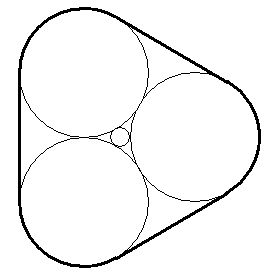
\includegraphics[]{i1.png} 
        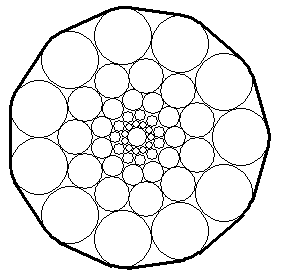
\includegraphics[]{i2.png} \\ 
    \end{center}
\end{figure}

The queen does not yet know how many stones there will be in each
circle nor how many circles of stones there will be.  To be prepared
for whatever she decides, write a program to calculate the sizes of
the stones in each circle and the length of the surrounding fence.
The radius of the central stone is to be one \emph{queenly} foot.

\section*{Input}

The first line of input contains a single integer $P$, ($1 \le P \le 1000$)
which is the number of data sets that follow.  Each data set should be
processed identically and independently.

Each data set consists of a single line of input.  It contains the
data set number, $K$, the number, $N$ ($3 \le N \le 20$), of stones in each
circle and the number, $M$ ($1 \le M \le 15$), of circles of stones around
the central stone.

\section*{Output}

For each data set there is a single line of output.  It contains the
data set number, $K$, followed by a single space which is then followed by
the radius (in queenly feet) of the stones in the outermost ring (to $3$
decimal places) which is followed by a single space which is then followed
by the length (in \emph{queenly feet}) of the fence (to $3$ decimal places).

